\subsection{Конструкция на платформата}

\subsection{Платформа с четири ротора}
\FloatBarrier

Платформата \autoref{fig:drone_construction} е конструирана от два метални П-образни профила, сключващи прав ъгъл помежду си и имащи пресечна точка в средата.
В края на профилите се намира по един безчетков постояннотоков мотор (без обратна връзка).
Перките са свързани директно (без трансмисия) за въртящата ос на моторите.
Батерията и контролният модул са позиционирани в средата на платформата.
Батерията се намира под пресечната точка на профилите.
Управляващото устройство е над пресеччната точка на профилите
върху изработена, като част от проекта, платформа.

При този начин на организиране на хардуера центърът на тежеста лежи под пресечната точка на профилите.


\begin{figure}[htpb!]
    \centering
    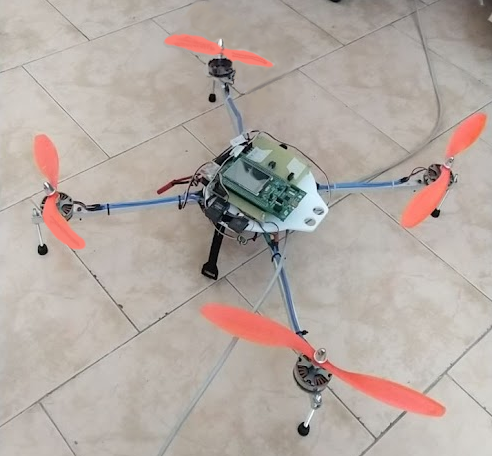
\includegraphics[width=0.5\textwidth]{drone_construction}
    \caption{Конструкция на платформата с четири ротора}
    \label{fig:drone_construction}
\end{figure}



\FloatBarrier
\subsection{Платформа за управление на ъгъл на завъртане}
\FloatBarrier

Платформата за управление на ъгъл на завъртане има за цел да ни позволи лесно и безаварийно да изпробваме алгоритмите за управление на ъгъл на завъртане.

Платфомрата \autoref{fig:balance_construction} е изградена от дърво.
Състои се от Т-образна основа с ограничители и въртяща част.
Основата е висока \(30cm\) и е съставена от два правоъгълни дървени профила (\(30x10x2.5cm\)), съединенин с винтове. 
Ограничителите ограничават максималния ъгъл, който въртящата част може да сключва с хоризонта в диапазона (\(\pm 40^{\circ}\)).
Оста на въртене представлява M8 болт.
Оста образува болтово съединение с основата, както и с лагерите на въртяащата част.
Въртящата част е съставена от правоъгълен дървен профил (\(60x2.5x3cm\)) с вложени два лагера 
(сачмен с дълбок канал \(8x22mm\), максимално статично натоварване \(138kg\) \cite{datasheet_bearing}),
като са пробити отвори за болтово съединяване на основите за безчетковите постояннотокови мотори,
както и отвори за болтово съединяване на основата на жироскопа и акселерометъра.
Останалите нужни компонении като \textit{ESC (Electronic Speed Controller)} за моторите са прикрепени към рамената на въртящата
част чрез кабелни превръзки (т.нар свински опашки), като е взето предвид балансиране на платформата
чрез разпределение на тежеста на допълнителните елементи.

\begin{figure}[htpb!]
    \centering
    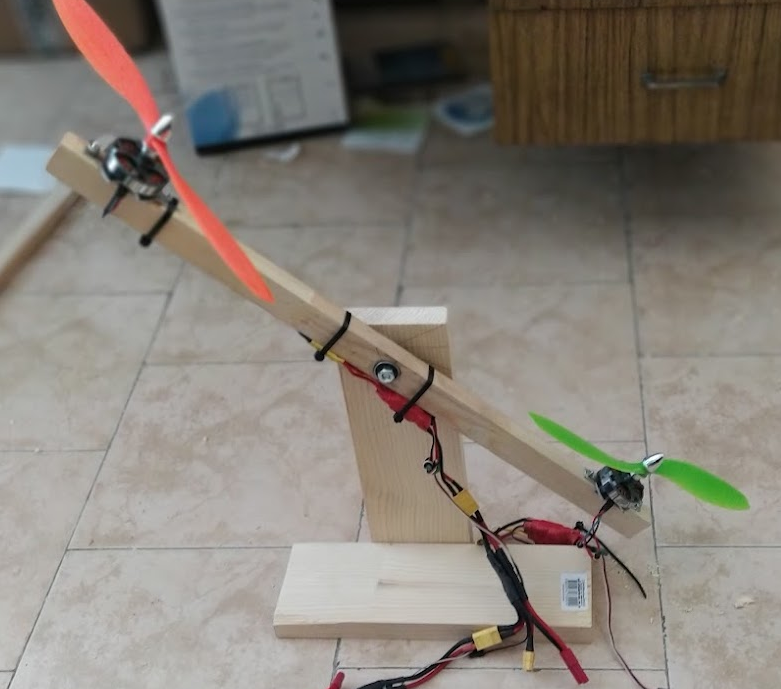
\includegraphics[width=0.7\textwidth]{balance_construction}
    \caption{Конструкция на платформата за управление на ъгъл}
    \label{fig:balance_construction}
\end{figure}

\FloatBarrier

